\chapter{Шаардлага ба төлөвлөлт}

\section{Функционал шаардлага (Functional Requirements)}
Системийн гүйцэтгэх үндсэн үйлдлүүдийг SRS стандартын дагуу \cite{ieee1998srs} дараах байдлаар тодорхойлов.
\begin{enumerate}[label=FR\arabic*.]
    \item \textbf{Тогтмол илэрхийлэлд суурилсан танилт}: Хэрэглэгчийн тохируулсан тогтмол илэрхийлэл ашиглан ирж буй зурвасыг автоматаар таньж, ангилах.
    \item \textbf{Харилцан ярианы ангиллын шошголол}: Харилцан яриа бүрт тухайн зурваст тохирох өнгөт шошго оноож, харагдах байдлыг ялгах.
    \item \textbf{Дасан зохицох хэрэглэгчийн харилцах цонхны дэмжлэг}: Нугалдаг төхөөрөмж нээгдэх үед хэрэглэгчийн харилцах цонхыг хоёр баганат харагдац руу гацалтгүйгээр шилжүүлэх.
    \item \textbf{Шудрах үйлдлийн тохиргоо}: Харилцан яриаг баруун, зүүн тийш шудрах үйлдлээр устгах, архивлах зэрэг үйлдлийг хурдан гүйцэтгэх.
    \item \textbf{Хугацааны бүлэглэлт}: Inbox дахь зурвасуудыг Өнөөдөр'', Өчигдөр'', Энэ сар'' гэсэн гарчиг дор автоматаар бүлэглэх.
\end{enumerate}

\section{Функционал бус шаардлага (Non-Functional Requirements)}
Системийн чанар болон найдвартай ажиллагааг хангах дараах шаардлагуудыг тавьсан:
\begin{itemize}
    \item \textbf{Гүйцэтгэл}: 1,000-аас дээш харилцан яриатай үед жагсаалт секундэд 60 frame хурдтай (smooth scroll) ажиллах.
    \item \textbf{Аюулгүй байдал}: Зурвасын агуулгыг гадагш дамжуулахгүй, бүх шүүлтүүрийг локал төхөөрөмж дээр (On-device) ажиллуулах.
    \item \textbf{Найдвартай байдал}: Room өгөгдлийн сангийн \cite{room_guide} шилжилт хийх үед хэрэглэгчийн өмнөх өгөгдөл алдагдахгүй байх.
    \item \textbf{Уян хатан байдал}: Шүүлтүүрийн дүрмийг хэрэглэгч хүссэн үедээ өөрчлөхөд систем бодит хугацаанд хариу үзүүлэх.
\end{itemize}

\section{Ажлын хүрээ (Scope Statement)}
Төслийн ажлын хүрээг \cite{clegg1994case} MoSCoW аргачлалаар эрэмбэлж тодорхойлов.
\begin{itemize}
    \item \textbf{Must-Have}: Тогтмол илэрхийллийн хөдөлгүүр, Room өгөгдлийн сангийн шилжилт, динамик хавтаслах систем.
    \item \textbf{Should-Have}: Нугалдаг төхөөрөмжийн хоёр баганат харагдацын тасралтгүй байдал, шудрах үйлдэл, зурваснуудыг насаар бүлэглэх.
    \item \textbf{Could-Have}: Зурвасын агуулгад тулгуурласан ухаалаг мэдэгдэл (Smart Notifications).
    \item \textbf{Won't-Have}: Cloud Backup, RCS (Rich Communication Services) дэмжлэг.
\end{itemize}

\section{Хөгжүүлэлтийн төлөвлөгөө (Development Plan)}
Хөгжүүлэлтийн ажлыг Iterative (Давталттай) аргачлалаар гүйцэтгэсэн бөгөөд доорх үе шатуудад хуваав:
\begin{enumerate}
    \item \textbf{I үе шат}: Суурь өгөгдлийн сангийн өргөтгөл болон тогтмол илэрхийллийн шүүлтүүрийн алгоритм хөгжүүлэлт.
    \item \textbf{II үе шат}: Хавтас удирдлагын систем болон шудрах үйлдлүүдийн UI хөгжүүлэлт.
    \item \textbf{III үе шат}: Нугалдаг төхөөрөмжийн дасан зохицох харагдац болон тасралтгүй байдлын логик.
    \item \textbf{IV үе шат}: Гүйцэтгэлийн оновчлол, тест ба чанарын баталгаажуулалт.
\end{enumerate}
\begin{itemize}
\section{Хэрэглээний тохиолдлын шинжилгээ (Use Case Analysis)} Системийн функционал шаардлагуудыг хэрэглэгчийн үйлдэл бүрээр нарийвчлан тодорхойлохын тулд хэрэглээний тохиолдлын диаграммыг (Зураг \ref{fig:usecase_diag}) боловсруулав. Энэхүү диаграмм нь хэрэглэгч болон системийн хоорондын харилцан үйлчлэлийг ерөнхий байдлаар харуулна.
\begin{figure}[H] \centering 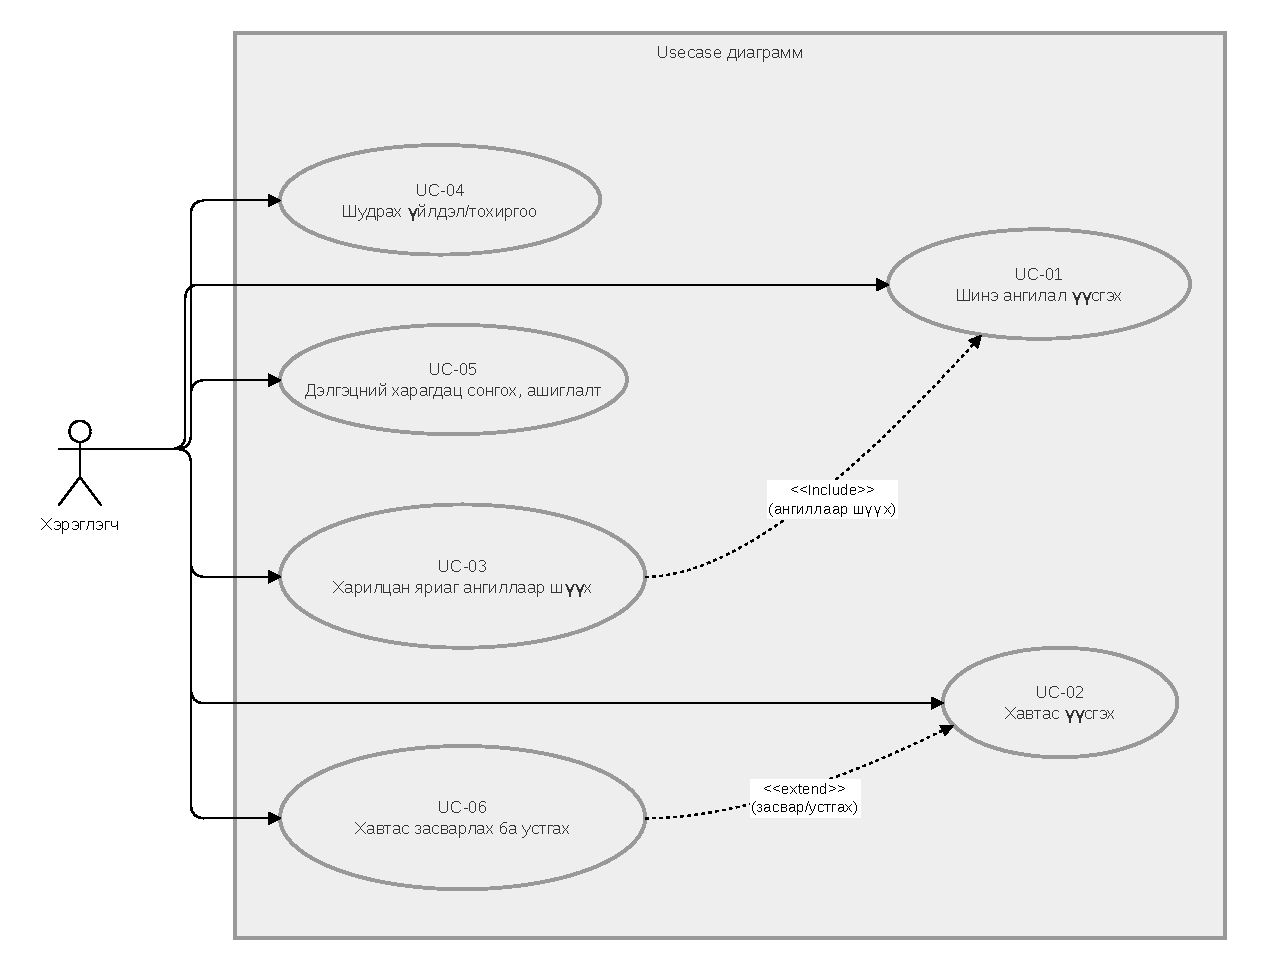
\includegraphics[width=0.85\textwidth]{Diagrams/usecase_diagram.drawio} \caption{Системийн хэрэглээний тохиолдлын диаграмм} \label{fig:usecase_diag} \end{figure}
    Дээрх диаграммд тусгагдсан үндсэн үйлдлүүдийн ажлын урсгал болон нөхцөлүүдийг дараах хүснэгтүүдээр дэлгэрэнгүй тайлбарлав.

% Хэрэглээний тохиолдол 1: Шошго үүсгэх
\begin{longtable}{|l|p{10.5cm}|}
    \caption{Хэрэглээний тохиолдол 1: Шошго үүсгэх} \label{tab:uc_create_category} \\
    \hline
    \textbf{ID / Нэр} & UC-01 / Шинэ шошго үүсгэх \\ \hline
    \textbf{Товч тайлбар} & Хэрэглэгч зурвас шүүх шинэ дүрэм (шошго) үүсгэж, нэр, өнгө болон шүүлтүүрүүдийг тохируулна. \\ \hline
    \textbf{Үйлдэгч} & Хэрэглэгч \\ \hline
    \textbf{Өмнөх нөхцөл} & Хэрэглэгч ``Шошго удирдах'' дэлгэцийг нээсэн байна. \\ \hline
    \textbf{Ажлын урсгал} &
    1. Хэрэглэгч ``+'' товчийг дарж үүсгэх цонхыг нээнэ. \newline
    2. Шошгоны нэрийг оруулж, жагсаалтаас өнгө сонгоно. \newline
    3. Шүүлтүүрийн төрлийг сонгоно: \newline
    \hspace{0.5cm} 3.1. Энгийн үг оруулах бол ``Энгийн үг нэмэх'' талбарт бичнэ. \newline
    \hspace{0.5cm} 3.2. Тогтмол илэрхийлэл (Regex) ашиглах бол дүрс дээр дарж паттерн оруулна. \newline
    4. Оруулсан өгөгдлийг шалгаж ``OK'' товчийг дарна. \\ \hline
    \textbf{Альтернатив} & Хэрэглэгч ``Cancel'' дарвал өөрчлөлт хадгалагдахгүй. Буруу тогтмол илэрхийллийн паттерн оруулбал систем алдаа заана. \\ \hline
    \textbf{Дараах нөхцөл} & Шинэ шошго баазад хадгалагдаж, зурвасууд шууд ангилагдана. \\ \hline
\end{longtable}

\vspace{1em}

% Хэрэглээний тохиолдол 2: Хавтас үүсгэх
\begin{longtable}{|l|p{10.5cm}|}
    \caption{Хэрэглээний тохиолдол 2: Хадгалсан харагдац (Хавтас) үүсгэх} \label{tab:uc_create_folder} \\
    \hline
    \textbf{ID / Нэр} & UC-02 / Хавтас үүсгэх \\ \hline
    \textbf{Товч тайлбар} & Хэрэглэгч өөрийн хэрэгцээнд тохирсон зурвасын харагдац (Хавтас) үүсгэж, доод навигацийн цэсэнд нэмнэ. \\ \hline
    \textbf{Үйлдэгч} & Хэрэглэгч \\ \hline
    \textbf{Ажлын урсгал} &
    1. Баруун дээд цэснээс ``Хавтас'' -> ``Харагдац үүсгэх'' сонгоно. \newline
    2. Хавтасны нэрийг бичиж, харагдах байрлал (index) болон өнгийг тодорхойлно. \newline
    3. ``OK'' товчийг дарж баталгаажуулна. \\ \hline
    \textbf{Дараах нөхцөл} & Шинэ хавтас доод навигацийн цэсэнд нэмэгдэж, хэрэглэгч тухайн хавтас руу автоматаар шилжинэ. \\ \hline
\end{longtable}

\vspace{1em}

% Хэрэглээний тохиолдол 3: Шошгоор шүүх
\begin{longtable}{|l|p{10.5cm}|}
    \caption{Хэрэглээний тохиолдол 3: Шошгоор шүүх} \label{tab:uc_filter_category} \\
    \hline
    \textbf{ID / Нэр} & UC-03 / Харилцан яриаг шошгоор шүүх \\ \hline
    \textbf{Товч тайлбар} & Хэрэглэгч үүсгэсэн хавтас доторх харилцан яриануудыг нэг болон хэд хэдэн шошгоор (Tag) шүүж харна. \\ \hline
    \textbf{Ажлын урсгал} &
    1. Хайх талбарын хажууд байрлах шүүлтүүрийн товчийг дарна. \newline
    2. Гарч ирэх жагсаалтаас нэг болон түүнээс дээш шошгыг сонгоно. \newline
    3. ``OK'' товчийг дарахад систем сонгосон шошгонд таарсан зурвасуудыг харуулна. \\ \hline
    \textbf{Дараах нөхцөл} & Жагсаалт шинэчлэгдэж, шүүлтийн төлөв хадгалагдана. \\ \hline
\end{longtable}

\vspace{1em}

% Хэрэглээний тохиолдол 4: Шудрах үйлдэл
\begin{longtable}{|l|p{10.5cm}|}
    \caption{Хэрэглээний тохиолдол 4: Шудрах үйлдлийн тохиргоо} \label{tab:uc_swipe_actions} \\
    \hline
    \textbf{ID / Нэр} & UC-04 / Шудрах үйлдлийн тохиргоо \\ \hline
    \textbf{Товч тайлбар} & Харилцан ярианы жагсаалтад зүүн эсвэл баруун тийш шудрахад хийгдэх үйлдлийг хэрэглэгч өөрөө сонгоно. \\ \hline
    \textbf{Ажлын урсгал} &
    1. Програмын ерөнхий тохиргооноос ``Шудрах үйлдэл'' хэсгийг нээнэ. \newline
    2. ``Эхнээс нь шудрах'' эсвэл ``Төгсгөлөөс нь шудрах'' сонголтыг дарна. \newline
    3. Боломжит үйлдлүүдээс (Устгах, Архивлах, Уншсан болгох г.м) нэгийг сонгоно. \\ \hline
    \textbf{Дараах нөхцөл} & Сонгосон үйлдэл тэр даруй хадгалагдаж, жагсаалт дээр ажиллаж эхэлнэ. \\ \hline
\end{longtable}

\vspace{1em}

% Хэрэглээний тохиолдол 5: Дэлгэцийн горим
\begin{longtable}{|l|p{10.5cm}|}
    \caption{Хэрэглээний тохиолдол 5: Дэлгэцийн харагдацын горим} \label{tab:uc_screen_view} \\
    \hline
    \textbf{ID / Нэр} & UC-05 / Screen View Mode сонгох \\ \hline
    \textbf{Товч тайлбар} & Нугалдаг төхөөрөмж эсвэл таблет дээр жагсаалт болон дэлгэрэнгүй хэсгийг хэрхэн харуулахыг тохируулна. \\ \hline
    \textbf{Ажлын урсгал} &
    1. Тохиргоо цэсний ``View mode'' хэсэгт орно. \newline
    2. ``Auto'', ``Single'', эсвэл ``Separated'' горимуудаас нэгийг сонгоно. \newline
    3. ``Auto'' горимд систем дэлгэцийн төлөвийг (Дэлгэц хаалттай/нээлттэй) мэдэрч автоматаар шилжинэ. \\ \hline
    \textbf{Дараах нөхцөл} & Програмын үндсэн дэлгэцийн бүтэц (layout) сонгосон горимын дагуу шинэчлэгдэнэ. \\ \hline
\end{longtable}

\vspace{1em}

% Хэрэглээний тохиолдол 6: Хавтас засварлах
\begin{longtable}{|l|p{10.5cm}|}
    \caption{Хэрэглээний тохиолдол 6: Хавтас засварлах ба устгах} \label{tab:uc_edit_folder} \\
    \hline
    \textbf{ID / Нэр} & UC-06 / Хавтас засах эсвэл устгах \\ \hline
    \textbf{Товч тайлбар} & Өмнө үүсгэсэн хавтасны мэдээллийг шинэчлэх эсвэл системээс бүрмөсөн устгана. \\ \hline
    \textbf{Ажлын урсгал} &
    1. Доод навигацийн цэс дээрх хавтасны дүрс дээр удаан дарна. \newline
    2. Мэдээллийг (нэр, өнгө, байрлал) засаад ``OK'' дарах эсвэл ``Delete'' товчийг сонгоно. \newline
    3. Устгах үйлдэл дээр систем дахин баталгаажуулалт асууна. \\ \hline
    \textbf{Дараах нөхцөл} & Өөрчлөлт хадгалагдах эсвэл хавтас навигацийн цэснээс алга болж хэрэглэгч үндсэн харагдац руу шилжинэ. \\ \hline
\end{longtable}

    \paragraph{Төслийн өргөтгөлүүдийн байршил:}
    Дээрх суурь бүтцэд хийсэн өргөтгөлүүд дараах сангуудад нэмэгдсэн:
    \begin{itemize}
        \item \textbf{Regex Filtering логик} – \texttt{messaging/} ба \texttt{extensions/} сангуудад нэмэгдсэн (жишээ нь \texttt{withAutoCategory()}, \texttt{isMessageMatchingCategory()}).
        \item \textbf{Foldable device support} – \texttt{activities/} (\texttt{MainActivity} two-pane логик) болон \texttt{helpers/} (\texttt{FoldableHelper}) хэсэгт хийгдсэн.
        \item \textbf{SavedViews (Folder) систем} – \texttt{models/} (\texttt{SavedView}, \texttt{SavedViewConfig}), \texttt{helpers/} (\texttt{SavedViewsStore}), \texttt{databases/} (Config өргөтгөл) зэрэгт шинээр нэмэгдсэн.
        \item \textbf{Category ба Regex дүрмийн UI} – \texttt{activities/}, \texttt{dialogs/}, \texttt{ui/} (Compose KeywordManager) сангуудад хийгдсэн.
    \end{itemize}
Хөгжүүлэлтийн явцад Git-ийн Feature Branch'' стратегийг \cite{vincent_git} ашиглаж, долоо хоног бүр явцын түүхийг баталгаажуулсан.
